%% LyX 2.4.0~RC3 created this file.  For more info, see https://www.lyx.org/.
%% Do not edit unless you really know what you are doing.
\documentclass[spanish,openright]{book}
\usepackage[serif]{libertinus}
\renewcommand{\sfdefault}{LibertinusSans-LF}
\renewcommand{\ttdefault}{LibertinusMono-TLF}
\renewcommand{\familydefault}{\rmdefault}
\usepackage[T1]{fontenc}
\usepackage{textcomp}
\usepackage[utf8]{luainputenc}
\usepackage[paperwidth=8.25in,paperheight=11in]{geometry}
\geometry{verbose,tmargin=2cm,bmargin=2cm,lmargin=2cm,rmargin=1.5cm}
\usepackage[skip=\medskipamount]{parskip}
\usepackage{graphicx}
\usepackage{rotfloat}

\makeatletter
%%%%%%%%%%%%%%%%%%%%%%%%%%%%%% User specified LaTeX commands.
% To ensure automatically inserted blank pages have no header/page number
\usepackage{emptypage}

% For avoid chapter number in sections/subsections
\renewcommand{\thesection}{\arabic{section}}
\renewcommand{\thesubsection}{\thesection.\arabic{subsection}}
\renewcommand{\thesubsubsection}{\thesubsection.\arabic{subsubsection}}

\makeatother

\usepackage{babel}
\addto\shorthandsspanish{\spanishdeactivate{~<>}}
\deactivatequoting

\begin{document}
\frontmatter

\thispagestyle{empty}
\vspace*{0.30\textheight}
\begin{center}
{\huge\textbf{MANUAL DE LOGÍSTICA ADUANERA Y COMERCIO EXTERIOR}}{\huge\par}
\par\end{center}

\cleardoublepage
\begin{center}
{\huge\textbf{MANUAL DE LOGÍSTICA ADUANERA }}{\huge\par}
\par\end{center}

\begin{center}
{\huge\textbf{Y COMERCIO EXTERIOR}}{\huge\par}
\par\end{center}

\begin{center}
\vspace*{0.35\textheight}
\par\end{center}

\begin{center}
{\large\textbf{JAIME ARMANDO PÉREZ}}{\large\par}
\par\end{center}

\begin{center}
\vspace*{0.45\textheight}
\par\end{center}

\begin{center}
\textbf{2026}
\par\end{center}

\thispagestyle{empty}

\textbf{MANUAL DE LOGÍSTICA ADUANERA Y COMERCIO EXTERIOR}\\
\textbf{Autor: }Jaime Armando Pérez

\medskip{}

© 2026 Jaime Armando Pérez. \\
Todos los derechos reservados.

Ninguna parte de este libro puede ser reproducida, almacenada en sistemas de recuperación ni transmitida por ninguna forma o medio (electrónico, mecánico, fotocopia, grabación u otros) sin el permiso previo y por escrito del titular del copyright.

\medskip{}

Esta edición ha sido publicada de forma independiente, 2026.

\textbf{ISBN} (Versión Impresa -- Tapa Dura): 979-81-937-3311-9\\
\textbf{ISBN} (Versión Digital/PDF): 978-62-897-5631-9\\
\textbf{Edición}: Primera Edición (Año 2026) -- Versión Tapa Dura

\medskip{}

\textbf{Diseño de Portada}: Jaime Armando Pérez\\
\textbf{Diagramación y Formato}: Luis Ernesto Garreta Unigarro

\medskip{}

\textbf{NOTA LEGAL Y DE EXENCIÓN DE RESPONSABILIDAD}

El contenido de este manual tiene fines estrictamente académicos y profesionales informativos en el área de la logística aduanera y el comercio exterior. Aunque el autor ha verificado exhaustivamente la normatividad y procedimientos vigentes a la fecha de publicación, las normativas aduaneras y de comercio internacional están sujetas a constantes modificaciones estatales e internacionales. Ni el autor ni la plataforma de distribución asumen responsabilidades por pérdidas o perjuicios derivados de la interpretación o aplicación práctica de la información contenida en esta obra

\cleardoublepage

\chapter*{Prefacio}

\addcontentsline{toc}{chapter}{Prefacio}

El comercio exterior es mucho más que una operación de compra o venta internacional: es un puente que conecta economías, culturas, oportunidades y crecimiento. Pero para que ese intercambio sea posible, se requiere una estructura técnica sólida que garantice que cada mercancía se movilice con orden, seguridad, eficiencia y cumplimiento. Esa estructura es, precisamente, la logística aduanera.

Este manual nace de la experiencia académica y práctica en el sector, con el objetivo de brindar al lector una guía clara, útil y aplicable sobre los procesos esenciales del comercio exterior y la gestión aduanera. Su enfoque busca integrar conocimiento normativo, visión operativa y herramientas prácticas, especialmente orientadas a la realidad colombiana.

A través de estas páginas, el lector encontrará una ruta de aprendizaje que le permitirá comprender los fundamentos, identificar riesgos, fortalecer su criterio técnico y desarrollar competencias para enfrentar con responsabilidad los desafíos de una operación aduanera moderna.

El propósito directo es aportar al crecimiento profesional de quienes se forman y trabajan en este campo, impulsando una cultura de legalidad, ética, control preventivo y excelencia operativa.

Finalmente, agradezco a quienes, desde la práctica operativa, la docencia y la experiencia institucional, nos permitieron la construcción de este conocimiento. Confío en que este manual sea una herramienta útil para el aprendizaje, la consulta permanente y el desarrollo de una gestión aduanera cada vez más eficiente y transparente.

\cleardoublepage

\chapter*{Introducción}

\addcontentsline{toc}{chapter}{Introducción}

La logística aduanera y el comercio exterior constituyen pilares esenciales para el desarrollo económico y la competitividad de Colombia en los mercados internacionales. En un entorno globalizado, caracterizado por el intercambio constante de bienes, servicios y capitales, la eficiencia en los procesos aduaneros se convierte en un factor determinante para facilitar las operaciones de exportación e importación, reducir costos logísticos y asegurar el cumplimiento normativo.

En el contexto colombiano, la logística aduanera integra un conjunto de procedimientos, regulaciones y actores que intervienen desde el ingreso o salida de mercancías, hasta su nacionalización o embarque hacia otros destinos. Instituciones como la Dirección de Impuestos y Aduanas Nacionales (DIAN), el Ministerio de Comercio, Industria y Turismo (MinCIT), y entidades como la Policía Fiscal y Aduanera (POLFA), juegan un papel fundamental en la vigilancia, control y facilitación del comercio legítimo.

La logística aduanera es uno de los componentes clave dentro de esta dinámica. Más allá de los simples trámites de importación y exportación, involucra la coordinación eficiente de diversos actores, como empresas transportadoras, agencias de aduanas, autoridades portuarias y aeropuertos, así como organismos regulatorios, con el objetivo de asegurar que las operaciones se lleven a cabo de manera ágil, segura y conforme a la normativa vigente. En este sentido, las reformas aduaneras implementadas en Colombia en los últimos años han buscado hacer frente a los retos de la modernización tecnológica, la transparencia y la lucha contra el contrabando. 

Las organizaciones actuales deben contemplar la posibilidad de desarrollar actividades referentes a la logística de carácter global, capaz de proveerse de materias primas y productos elaborados y provenientes de cualquier país que pueda ofrecerlos en condiciones favorables, tanto técnica como económicas, y de características ambientales sostenibles.

En un mundo globalizado, el comercio exterior se ha convertido en un pilar fundamental para el desarrollo económico de los países, y Colombia no es la excepción. Con una economía en constante evolución y un creciente interés por expandir sus mercados internacionales, el país ha puesto especial énfasis en mejorar su infraestructura y procedimientos aduaneros para facilitar el flujo de bienes y servicios hacia y desde el exterior.

La gestión aduanera, en el marco del comercio exterior o internacional, abarca una diversidad de operaciones que la hacen sumamente compleja. Coexisten operaciones comerciales de importación, exportación, regímenes especiales y tránsito de mercancías, junto con la logística del transporte, almacenaje y tangencialmente con la distribución, que operan en el cumplimiento de las normas fiscales, de control de seguridad y de política comercial exterior. Para los agentes que intervienen en el comercio internacional, ello significa disponer de una serie de servicios, infraestructuras y terminales logísticas adecuados para la circulación y el almacenamiento de mercancías, así como aplicar los procedimientos aduaneros que permitan atender las necesidades del mercado de manera eficaz, pues en un mercado abierto el más eficaz disfruta de ventaja comparativa frente a los demás. 

La articulación entre logística aduanera y comercio exterior permite garantizar el flujo seguro y oportuno de mercancías, optimizar los tiempos de operación y promover la inserción del país en cadenas globales de valor. Comprender estos elementos es esencial para profesionales, empresas y estudiantes que participan o aspiran a participar en actividades de comercio internacional, dado que un manejo adecuado de la normativa y los procedimientos es clave para competir en un mercado dinámico y altamente regulado.

Para un mejor entendimiento de los procesos de administración de importaciones y exportaciones de bienes y servicios, la globalización ha hecho que las operaciones logísticas inmersas en estos procesos tengan una realidad constante, por lo tanto, se han de tener muy presentes el conocimiento y el cumplimiento de las normas legales relativas a la gestión aduanera, junto con las operaciones conexas de transacciones financieras en divisas y los servicios de transporte internacional, almacenamiento y tráfico de mercancías.

En este contexto, para afrontar los retos derivados del comercio con mercados externos, las empresas precisan que sus gestores y directivos posean amplios conocimientos que permitan disponer de las herramientas necesarias para emprender tales actividades. Para ello será necesario, por una parte, que conozcan los deberes, obligaciones y responsabilidades de la gestión aduanera en referencia al intercambio de mercancías, producto de las compraventas con el exterior; y, por otra parte necesitarán contar con la ayuda de profesionales, internos o externos, capacitados en las técnicas del comercio internacional, que se sumen en el logro de los objetivos empresariales planteados en cuantas operaciones hayan de ejecutarse para que las mercancías lleguen a su destino en la forma más eficiente posible.

Las legislaciones y los acuerdos que regulan las transacciones internacionales, aunque son de origen diverso, poseen objetivos comunes y constituyen un marco de cooperación comercial sobre principios de concertación, que se adaptan progresivamente a os nuevos objetivos económicos, políticos y sociales. De igual modo, las instituciones regionales han evolucionado en función de sus cometidos y ha consolidado la integración comercial de los estados miembros, mientras los gobiernos de otros estados han formalizado acuerdos de cooperación con el objetivo de competir en el mercado mundial.

Las empresas y la administración pública han de disponer de los recursos necesarios para afrontar los retos del comercio internacional: las primeras, mediante la fabricación y la oferta de bienes y servicios según los requisitos solicitados por los clientes; la segunda, velando por el cumplimiento de las reglamentaciones de manera ágil. Ambas partes han de colaborar en el mismo objetivo, que no es otro que el desarrollo empresarial productivo, iniciando en el seno de la empresa y con repercusión final en el producto interno bruto (PIB) de cada país. Si alguna de las dos partes no cumple adecuadamente su cometido, la otra sufre las consecuencias, que finalmente se trasladan al conjunto de la sociedad mediante la disminución o el incremento de la renta nacional.

\cleardoublepage

\chapter*{Objetivos}

\addcontentsline{toc}{chapter}{Objetivos}

\section*{Objetivo General}

Analizar los fundamentos, procedimientos, normatividad y actores que intervienen en la logística aduanera y el comercio exterior colombiano, con el fin de comprender su importancia en la facilitación del intercambio internacional de bienes y en la competitividad del país.

Ofrecer una visión integral sobre la logística aduanera y el comercio exterior en Colombia, analizando tanto el marco regulatorio como los procesos operativos que impactan el desarrollo de estas actividades. Se abordarán ejemplos prácticos de manera física y sistemática, con el fin de proporcionar una herramienta de referencia para profesionales del área, estudiantes y todos aquellos interesados en comprender las dinámicas comerciales y aduaneras que configuran el panorama económico colombiano.

\section*{Objetivos Específicos}
\begin{enumerate}
\item Describir el marco normativo que regula las operaciones de comercio exterior en Colombia, incluyendo las disposiciones aduaneras, tributarias y los tratados internacionales vigentes.
\item Explicar los procesos operativos y logísticos asociados a la importación, exportación, tránsito y almacenamiento de mercancías en el territorio aduanero nacional.
\item Identificar los actores públicos y privados que intervienen en la logística aduanera, así como sus responsabilidades y funciones dentro de la cadena logística internacional.
\item Analizar los principales instrumentos de facilitación del comercio implementados en Colombia, como las zonas francas, el Operador Económico Autorizado (OEA) y los acuerdos comerciales.
\item Evaluar la incidencia de la logística aduanera en la competitividad empresarial y en la integración del país a los mercados globales.
\item Reconocer los retos actuales del sistema aduanero colombiano, incluyendo la transformación digital, la seguridad en la cadena logística y la lucha contra el comercio ilícito.
\end{enumerate}
\cleardoublepage

\tableofcontents{}

\cleardoublepage

\listoffigures

\cleardoublepage

\mainmatter

\chapter{Breve Historia del Comercio Exterior}

\section{Comercio Exterior Global}

El comercio es una de las actividades económicas de mayor antigüedad, pues se inició con el hombre mismo.

El comercio se ha considerado como el intercambio, entre dos o más individuos, de bienes y servicios que les son necesarios para satisfacer sus necesidades. 

Dicha actividad surge cuando el hombre advierte la dificultad o la imposibilidad de producir determinados bienes que otros poseen y que pueden ser adquiridos mediante el cambio; es así como aparece la forma primitiva de cambio, el trueque. 

La Academia Española nos dice que el comercio es la negociación que se hace comprando, vendiendo o permutando unas cosas por otras. 

Obviamente que en el presente la técnica ha evolucionado el primitivo comercio de los pueblos con lo que ahora conocemos como comercio en línea. Esto ha significado la ampliación en el volumen de transacciones debido a la inmediación geográfica de las naciones. Podemos decir que cuando la zona de intercambio sobrepasó las fronteras nacionales surgió el comercio internacional. 

El término “comercio exterior” es generalmente atribuido a John Stuart Mill, quien lo uso para sustituir el término “comercio internacional”. Este último, primeramente, usado por Bentham en 1780, puede crear ciertos problemas para la definición del concepto que nos interesa. Estrictamente hablando, las naciones como tales no surgieron sino hasta el período del Renacimiento (siglos XV y XVI); sin embargo, resultaría extraño decir que el término “comercio internacional”, esto es, el intercambio de bienes o servicios entre diferentes pueblos surgió en la tardía época medieval. Por ello es conveniente hacer una referencia, tan breve cómo es posible dentro de una introducción, al comercio que se desarrolló en los pueblos antiguos.

\subsection{Orígenes}

Quedó establecido que el comercio apareció con el hombre mismo. 

Con la finalidad de saciar las necesidades humanas, las causas motoras del comercio fueron la desigualdad en los recursos naturales del hábitat y la especialización en la producción. 

El primer comercio fue terrestre, más después fue fluvial y luego marítimo y es en este medio donde se caracteriza en primer término el comercio exterior. 
\begin{description}
\item [{Los~Fenicios.}] Estos últimos llegaron a dominar el comercio desde las costas de mar mediterráneo La historia nos dice que dentro del mundo occidental se considera a los pueblos mesopotámicos, a los egipcios y los fenicios como los pioneros del comercio hasta las costas occidentales del norte de África y las costas europeas, extendiendo su dominio hasta las costas del mar báltico.
\item [{Los~Griegos.}] La cultura helénica logró su gran desarrollo debido a la atención que le prestó a la navegación y al comercio que los fenicios venían desarrollando, participando en sus relaciones comerciales con Cartago. La competencia comercial dio motivo a varios enfrentamientos bélicos.

Los griegos finalmente dominaron el mundo conocido hasta entonces. Su dominio duró tres siglos para ser desplazados por los romanos. 
\item [{Los~Romanos.}] Los romanos fueron los más importantes constructores de caminos para fines militares, obras que también fueron usadas para el comercio; además desarrollaron vías marítimas, pues contaban con una impresionante flota de galeras para transportar las mercancías desde sus colonias hasta Roma y viceversa. Los códigos teodosianos y justinianos contienen disposiciones relativas al tráfico comercial.

En el cenit de su imperio, ellos controlaban toda Europa occidental, incluyendo las islas británicas, el medio oriente y la parte norte de África. Roma era el centro de intercambio de las diferentes mercancías que llegaban de todas sus provincias. 
\item [{Las~Ligas~de~Ciudades~Comerciales.}] Durante las últimas etapas de la edad media, el comercio volvió a florecer, siendo este el motivo del surgimiento de varias ligas ciudades. 

Su objeto primordial era lograr la seguridad de sus naves y sus rutas comerciales en contra de los piratas y de los nobles feudales.

Existieron varias ligas: la Liga Romana con las ciudades del bajo Rhin y del Danubio, la Liga Suava (Nuremberg y Ausburgo en el siglo XIV.

La más importante fue la Liga Hanseática de 1241 que fue fundada por las ciudades alemanas de Hamburgo y Lubeck.

Esta Liga fue tan poderosa como un Estado, pues mantuvo un ejército y fuerza naval; entró en guerra con naciones y realizó tratados de paz con ellas, imponiendo sus condiciones en algunas ocasiones. Mantuvo enviados diplomáticos y cónsules en otros países para agilizar sus transacciones comerciales. Así mismo, concedía préstamos a gobiernos que la favorecían por medio de concesiones, exenciones o monopolios en las áreas de pesca, minería, manufacturas y agricultura.

En sus mejores tiempos, esta liga dominó el comercio en el Mar de Norte y en el Mar Báltico y fue un factor de influencia entre la etapa feudal y la renacentista.

Como la mayoría de las instituciones de esta época, tuvo un importante matiz religioso, participando activamente en las Cruzadas.

Las pugnas entre las diversas ciudades que la integraban, y la consolidación del Estado alemán, la llevaron a su desintegración.
\item [{España.}] Durante el imperio español, el comercio exterior de este país fue exclusivamente mercantilista, es decir, que dependió de la explotación y exportación de oro y plata, prohibiendo que sus colonias comerciaran con otros países entre sí, lo cual detuvo el progreso de estas posesiones y su debilitamiento económico
\item [{Inglaterra.}] Este país al invadir la India y al crear sus colonias en la América del Norte amplió su economía hasta convertirse en una potencia económica.
\end{description}

\subsection{Desafíos y Tendencias Actuales}

A medida que avanzamos en el siglo XXI, el comercio internacional enfrenta desafíos como tensiones comerciales entre las principales potencias, la pandemia de COVID-19 que afectó las cadenas de suministro globales y la creciente preocupación por cuestiones como el cambio climático y la sostenibilidad.

\subsection{Globalización}

A finales del siglo XX y principios del siglo XXI, la globalización aceleró el comercio internacional. Los avances en tecnología de la información, el transporte y las comunicaciones redujeron las barreras comerciales. Las cadenas de suministro se volvieron más complejas y las empresas buscaron mercados internacionales para expandirse.

En resumen, el comercio exterior global ha evolucionado a lo largo de los siglos, desde las antiguas rutas comerciales hasta la compleja red de intercambios que caracteriza la economía Mundial actual.

\begin{sidewaysfigure}
\begin{centering}
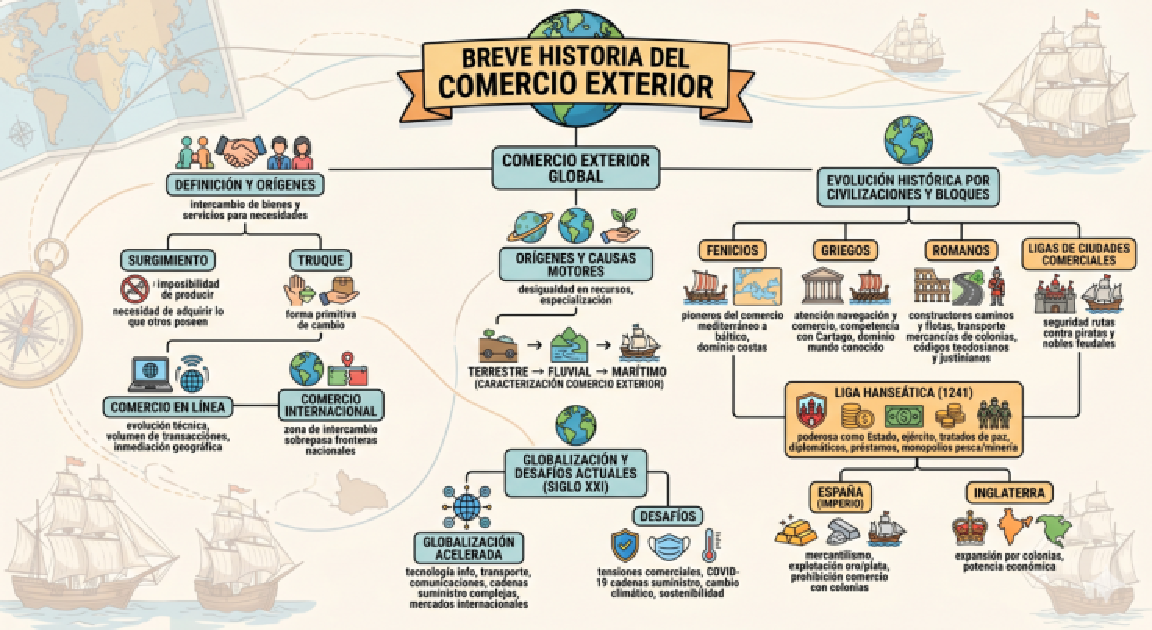
\includegraphics[width=24cm]{imagenes/image01-HistoriaComercio}
\par\end{centering}
\caption{\textbf{Breve Historia del Comercio Exterior Global.}}

\begin{centering}
Fuente: Elaboración propia (2025)
\par\end{centering}
\end{sidewaysfigure}


\section{Breve Historia del Comercio Exterior Colombiano}

El comercio exterior de Colombia tiene raíces que se remontan a la época precolombina, cuando las poblaciones indígenas intercambiaban bienes entre sí. Sin embargo, el comercio exterior formal comenzó a tomar forma durante la colonización española en el siglo XVI. En ese periodo, Colombia, como parte del Virreinato del Nuevo Reino de Granada, estaba vinculada principalmente a la economía española a través de la exportación de productos como oro, esmeraldas, café y tabaco.

Después de obtener su independencia en 1810, Colombia continuó exportando productos agrícolas, pero el comercio exterior experimentó cambios significativos a lo largo del siglo XIX y principios del siglo XX. Durante este período, el país diversificó sus exportaciones y comenzó a incluir productos como café, banano, flores, y productos derivados del petróleo.

En 1833 Se llevaron a cabo los primeros canales de exportación en el país, exportando tabaco desde Ambalema a Inglaterra, y en 1859 una de las primeras firmas extranjeras que exportó tabaco colombiano fue Powles, Gower \& Co

Con la presidencia de Carlos Lleras Restrepo en 1967, se introdujo en el país el Estado Aduanero y Control Cambiario, a su vez se creó la Ley 444 de 1967 denominada Plan de Promoción de Importación y Exportación (Plan Vallejo), a través del cual se puede importar materia prima, insumos, partes, repuestos y bienes de capital con exención total o parcial de tributos aduaneros, con destino a ser transformado en Colombia y posteriormente exportado. Por medio de la Ley 444 se estableció al Banco de la República como el único ente para ejercer el control cambiario.

En la presidencia de Misael Pastrana Borrero 1972, se creó el Abono Tributario, ahora denominado CERT (Certificado de Reembolso Tributario), este como incentivo del Estado para los exportadores en los pagos impositivos.

En el gobierno de Virgilio Barco 1982, se aplicaron flexibilizaciones sobre los productos importados: 80\% de productos son de libre importación (anteriormente solo el 10\% de la mercancía se podía importar sin el visto bueno del Gobierno), 5\% prohibida importación (anteriormente la limitante estaba en el 30\%. Aplica para la industria militar principalmente), 15\% con licencia previa (antes estaba en el 60\%). Por otra parte, se aplicaron disminuciones de aranceles, que estaban en un 80\% y 120\%, para pasar a un 5\% y 20\%.

Como presidente César Gaviria en 1991, se da la creación de la nueva constituyente y la gran reestructuración del comercio exterior, introduciendo nuevas instituciones como Mincomex, Bancoldex, DIAN (antes DAN y DIN), Consejo Superior de Comercio Exterior y los Intermediarios del Mercado Cambiario. A su vez se establece la libre tenencia y posesión de divisas.

Nace Procolombia en 1992 que es la entidad encargada de promover el Turismo, la Inversión Extranjera en Colombia, las Exportaciones no minero energéticas y la imagen del país en el exterior

En 2011 la economía colombiana se internacionaliza con nuevas normativas que permitieron multiplicar por ocho las exportaciones y la inversión extranjera. Las exportaciones pasaron de USD7.244 millones en 1991 a USD56.954 millones en 2011.

Actualmente se han dado grandes avances con importantes inversiones en base tecnológico. La DIAN cuenta con un sistema informático robusto, como lo es el SYGA (importaciones) y el MUISCA (exportaciones y tributos), además el Ministerio de Comercio cuenta con el VUCE (Ventanilla Única del Comercio Exterior) que agiliza trámites de permisos y registro de importaciones. De otro lado se ha dado la introducción de nuevas figuras que apoyan el comercio exterior como es el caso de las zonas francas y las comercializadoras internacionales.

El nuevo milenio trajo consigo una mayor globalización y la firma de tratados de libre comercio con varios países y regiones, como Estados Unidos, la Unión Europea y países de América Latina. Estos acuerdos buscaban ampliar las oportunidades comerciales y mejorar la competitividad de los productos colombianos en los mercados internacionales.

El comercio exterior de Colombia sigue siendo fundamental para su economía. Los principales socios comerciales incluyen Estados Unidos, China y países de la región latinoamericana. Las exportaciones colombianas siguen siendo diversas, abarcando productos como petróleo, café, flores, carbón, esmeraldas y textiles.

Es importante destacar que el comercio exterior de Colombia ha enfrentado desafíos, como la volatilidad de los precios de los productos básicos y los cambios en las condiciones económicas globales. Sin embargo, el país continúa adaptándose y buscando nuevas oportunidades para fortalecer su posición en el escenario internacional.

El comercio exterior de Colombia en el siglo XXI ha experimentado transformaciones significativas, impulsadas por cambios económicos, acuerdos comerciales, y fluctuaciones en los mercados globales. A continuación, se presentan algunos de los hitos y tendencias más importantes.

\subsection{Acuerdos Comerciales}

Colombia ha venido estructurando una política de integración económica abierta, en virtud de la cual ha logrado acercarse a un número cada vez mayor de mercados extranjeros. De manera particular para el ámbito latinoamericano, esta integración se ha dado en el marco de la Comunidad Andina (CAN), la Alianza del Pacífico y la Asociación Latinoamericana de Integración (ALADI).

\subsection{Crecimiento de Exportaciones No Tradicionales}

Durante la primera década del siglo XXI, Colombia comenzó a diversificar su oferta exportadora más allá del petróleo y el carbón, incluyendo productos agrícolas como flores, café especial, y frutas exóticas.

\subsection{Impacto de la Caída de los Precios del Petróleo (2014-2015)}

La caída de los precios del petróleo afectó significativamente las exportaciones colombianas, dado que los hidrocarburos representan una parte considerable de los ingresos por exportaciones. Esto obligó al país a acelerar sus esfuerzos de diversificación económica.

\subsection{Fortalecimiento del Sector Agroindustrial}

Productos como el café, las flores y el banano continuaron siendo fundamentales, pero también se impulsó la exportación de nuevos productos como aguacates y berries.

\subsection{Inversión en Infraestructura}

La inversión en infraestructura, especialmente en puertos y carreteras, ha sido crucial para mejorar la competitividad de Colombia en el comercio exterior.

\subsection{Impacto del COVID-19}

La pandemia de COVID-19 tuvo un impacto profundo en el comercio mundial, y Colombia no fue la excepción. Las exportaciones se redujeron significativamente en 2020, pero comenzaron a recuperarse en 2021 con la reactivación económica global.

\subsection{Nuevas Estrategias de Diversificación}

Colombia ha continuado enfocándose en la diversificación de sus exportaciones. Productos como el cannabis medicinal, los productos de tecnología, y el sector servicios (incluyendo BPO y TIC) han ganado relevancia.

\subsection{Mercados Emergentes}

En los últimos años, Colombia ha puesto énfasis en fortalecer relaciones comerciales con mercados emergentes en Asia y África, buscando reducir su dependencia de Estados Unidos y Europa.

\subsection{Tecnología y Sostenibilidad}

La adopción de tecnologías avanzadas y prácticas sostenibles está en la agenda para hacer que las exportaciones colombianas sean más competitivas y amigables con el medio ambiente.

\subsection{Infraestructura y Logística}

El gobierno y el sector privado están invirtiendo en mejorar la infraestructura logística para reducir costos y tiempos de exportación, haciendo a Colombia un jugador más fuerte en el comercio global.

En resumen, el comercio exterior de Colombia en el siglo XXI ha sido dinámico, enfrentando desafíos, pero también aprovechando oportunidades para diversificar y expandir su presencia en el mercado global.

\begin{sidewaysfigure}
\begin{centering}
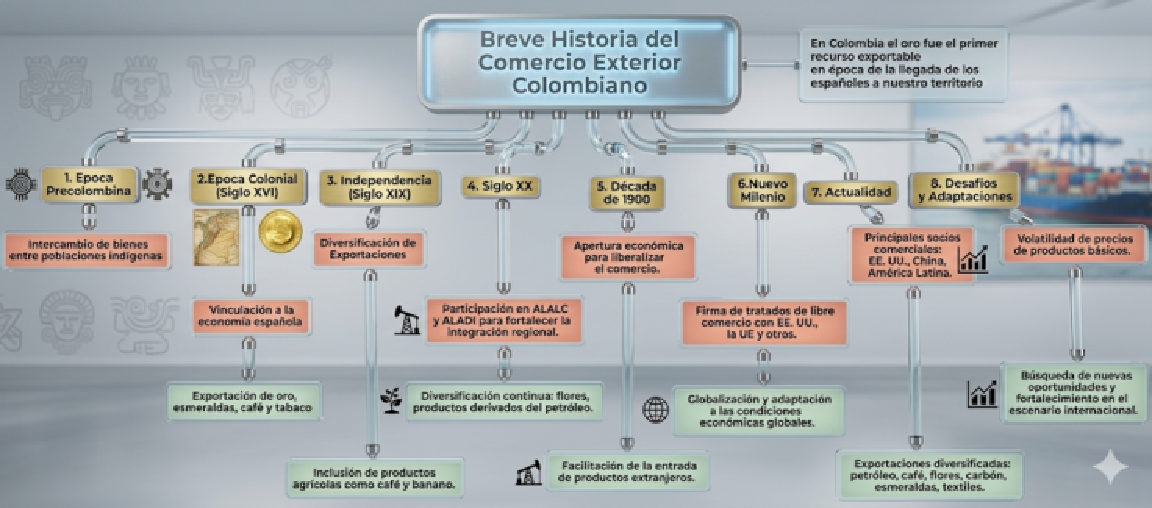
\includegraphics[width=24cm]{imagenes/image02-HistoriaComercioColombia}
\par\end{centering}
\caption{\textbf{Breve Historia del Comercio Exterior Colombiano}.}

\centering{}Fuente: Elaboración propia (2025)
\end{sidewaysfigure}

\begin{sidewaysfigure}
\begin{centering}
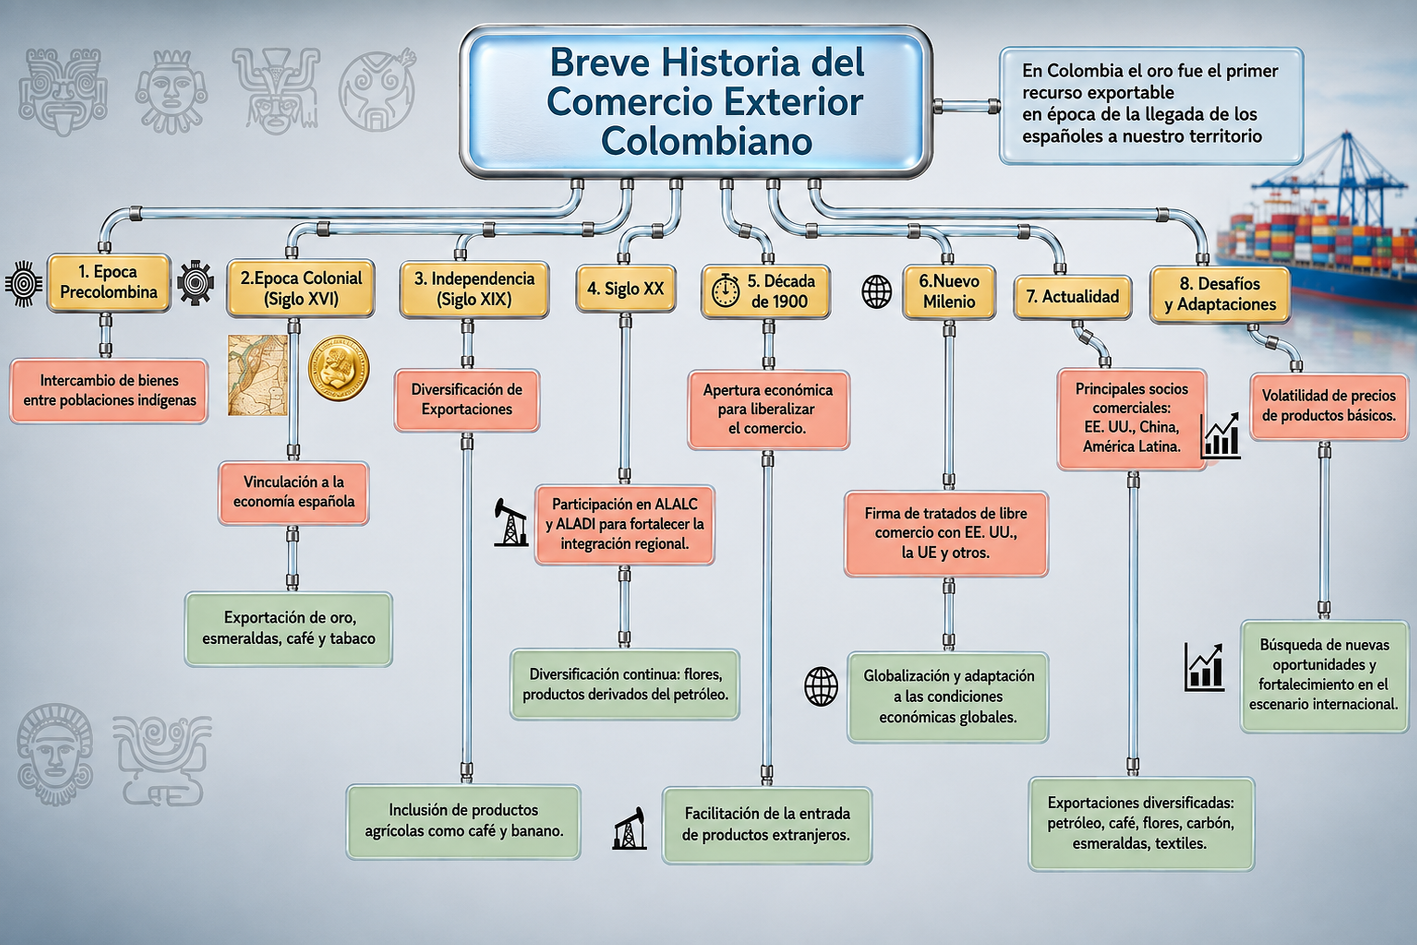
\includegraphics[width=24cm]{imagenes/image02-HistoriaComercioColombia-300dpi}
\par\end{centering}
\caption{\textbf{Breve Historia del Comercio Exterior Colombiano}.}

\centering{}Fuente: Elaboración propia (2025)
\end{sidewaysfigure}


\chapter{Factores y Sectores de Producción}

\section{Factores de Producción}

Los factores de producción son los recursos que se utilizan en el proceso de producción de bienes y servicios. Los principales factores de producción son tierra, trabajo, capital y habilidades empresariales.

\section{Relación los factores de producción con el comercio internacional}

Tierra. La disponibilidad y calidad de la tierra pueden afectar la producción de bienes agrícolas, lo que a su vez puede influir en la participación de un país en el comercio internacional de alimentos y productos agrícolas.

Trabajo. La mano de obra es un factor crucial en la producción de bienes y servicios. Los países con una fuerza laboral educada y capacitada pueden especializarse en la producción de bienes que requieren habilidades específicas. El comercio internacional permite a los países aprovechar las diferencias en los costos laborales y especializarse en la producción eficiente de ciertos bienes.

Capital. El capital, que incluye la maquinaria, tecnología y la infraestructura, influye en la capacidad de un país para producir bienes y servicios de manera eficiente. En el comercio internacional, la movilidad del capital puede permitir que las empresas busquen las condiciones más favorables para la inversión y la producción.

Habilidades Empresariales. Relación con el comercio: La capacidad de gestión y dirección de las empresas es un factor crítico en la producción eficiente. Los empresarios exitosos pueden identificar oportunidades en el mercado internacional y gestionar eficazmente las operaciones transfronterizas.

En el contexto del comercio internacional, surge el concepto de ventaja comparativa, propuesto por David Ricardo. Este concepto sugiere que los países se benefician al especializarse en la producción de bienes y servicios para los que tienen una ventaja comparativa (menores costos de oportunidad). El comercio internacional permite a los países aprovechar sus recursos de manera eficiente, ya que no todos los países tienen los mismos recursos en la misma cantidad o calidad.

Además, los acuerdos comerciales y la globalización han facilitado el movimiento de factores de producción a través de las fronteras, permitiendo una asignación más eficiente de estos recursos a nivel mundial.
\end{document}
